\documentclass[10pt, compress]{beamer}
\XeTeXlinebreaklocale "ja"
\XeTeXlinebreakskip=0em plus 0.1em minus 0.01em

\usetheme[usetitleprogressbar]{m}

\usepackage{booktabs}
\usepackage{minted}
\usepackage{fontawesome}
\usepackage{gnuplot-lua-tikz}
\usepackage{tcolorbox}

%%% user macro
\definecolor{links}{HTML}{DB4D6D} % NAKABENI
\hypersetup{colorlinks,linkcolor=,urlcolor=links}

%\tcbset{
%	width=.9\linewidth
%}

\newcommand{\ehref}[2]{\href{#1}{#2 \hspace{-.2em}{\scriptsize\faExternalLink}}}
%\newcommand{\eurl}[1]{\url{#1{\scriptsize \hspace{-.2em}\faExternalLink}}}
%%%

\usepgfplotslibrary{dateplot}

\usemintedstyle{trac}

\title{NICにおけるPCI Express性能の計測}
\subtitle{}
\date[\today]{}
%\author{Name (\ehref{http://twitter.com/twitter}{\faTwitter  twitter})}
\author{Yohei Kuga@KEIO Univ}
\institute{高速PCルータ研究会 2015/5}

\begin{document}

\maketitle

%% -------------------------------------------------- %%

\begin{frame}[fragile,t]{今日の話}
\begin{enumerate}
\item PCIe NICの基礎体力測定
\item ざっくばらんにFPGA開発ネタ
	\begin{itemize}
	\item FPGA+SystemVerilogで合成可能なパケット処理を考える
	\item その他のFPGA NIC実装
	\end{itemize}
\end{enumerate}
\end{frame}

%% -------------------------------------------------- %%

\begin{frame}[fragile,t]{Motivation}

ネットワークを高機能化するためにNICを自由に拡張したい
\vspace{.5em}

最近のDC+SW界隈 (Kernel bypass/Unikernels) に比べて,ネットワークHWはまだまだユーザ拡張性が低い
\vspace{-.5em}
\begin{itemize}
\item 現在のOffload機能はL2\~{}L4パケットヘッダ操作が主流
    \begin{itemize}
        \item Capsulation, CSUM, TCP など
    \end{itemize}
\item Programmable NICの検討は始まっている
\end{itemize}
\vspace{.5em}

"NICがProgrammableであること"が最初の一歩
\vspace{-.5em}
\begin{itemize}
\item ヘッダやFIB操作はProgrammable NICやNPUで実現可能
\item ペイロード操作/Interrupt/PCIe/遅延制御などを直接触りたいならFPGA NICが有力
\end{itemize}

\end{frame}

%%%%%%%%%%%%%%%%%%%%%%%%%

\begin{frame}[fragile,t]{今回のチャレンジ}

前回: シングルポート1GE NIC
\vspace{-.5em}
\begin{itemize}
\item Lattice ECP3 versa kit (1GEx2 + PCIe1.1)
\item PCIE-TX: PIO write + Write combining, RX: DMA write
\item Linux Driver and Timestamp機能
\end{itemize}

\vspace{1em}

今回: マルチポート10GE NIC
\vspace{-.5em}
\begin{itemize}
\item KC705 (10GEx4 + PCIe gen2 x8) or NetFPGA-SUME
\item PCIE: TX: DMA read, RX: DMA write
\item 性能目標: 少なくとも10G 2ポートはline rate出したい
\end{itemize}

\end{frame}

%%%

\begin{frame}[fragile,t]{FPGA NICのどこらへんが難しいのか}

いまのところ \textbf{マルチポート} らへんが課題
\vspace{-.5em}
\begin{itemize}
\item Ethernetポートは増やせても使えるPCIe帯域は共通
\item だめ回路ではマルチポートで性能がだせない可能性がある
\end{itemize}

\vspace{.5em}

しかしマルチポートNICのPCIe利用帯域の見積もりは難しい
\vspace{-.5em}
\begin{itemize}
\item ネットワークではマルチポート送受信利用が前提だがPCIeは共有
\item マルチポートEthernet利用時のTLP送信待ち時間が課題
\item マルチポート40GE/100GE NICがきびしい理由を計測から考える
\end{itemize}

\textcolor{blue}{今回は,市販NICでPCIeの現実に使える利用可能帯域を計測}
%\item あと,ここ1,2年で使えう用になったsystemverilogがとてもよかったので,その話もあとで少しだけ

\end{frame}

%%%%%%%%%%%%%%%%%%%%%%%%%

\begin{frame}[fragile,t]{計測のねらい}

\begin{itemize}
\item Ethernetの性能を最大限出すために,現実的なPCIeの利用可能帯域を探りたい
\item 一方で,市販NICはPCIe帯域に余裕を持って設計されているため,計測方法に工夫が必要
\item 今回はIntel x520-SR2 (10GE x2)を用いて計測
\end{itemize}
\vspace{-1em}

\begin{table}
\small{Intel 82599: Host Interface Features\footnotemark}
\begin{tabular}{l|l}
	\toprule
	PCIe Host Interface &  PCIe gen2 (2.5GT/s, 5GT/s)\\
	Number of Lanes & x1, x2, x4, x8\\
	\bottomrule
\end{tabular}
\end{table}

意図的にNIC PCIeの使用レーン数を絞ることでThroughputを計測

\footnotetext[1]{\ehref{http://www.intel.com/content/dam/www/public/us/en/documents/datasheets/82599-10-gbe-controller-datasheet.pdf}{(PDF) Intel 82599 10 GbE Controller Datasheet}}
\end{frame}

%%%%%%%%%%%%%%%%%%%%%%%%%

\begin{frame}[fragile,t]{計測環境}
\vspace{-1em}
\begin{table}
\begin{tabular}{l|l}
	\toprule
	Host CPU & Intel Core i7 4770\\
	NIC & Intel x520-SR2\\
	\midrule
	OS & BSD Router 1.55 (FreeBSD 10.1-RELEASE-p8)\\
	Tool & netmap pkt-gen\\
	\bottomrule
\end{tabular}
\end{table}

\vspace{-1em}
\begin{figure}
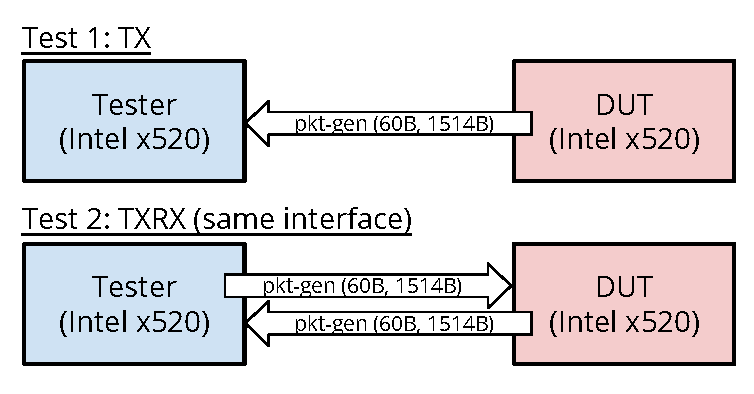
\includegraphics[width=.9\textwidth]{fig/test.pdf}
\end{figure}

\end{frame}


%%%%%%%%%%%%%%%%%%%%%%%%%

\begin{frame}{テープを使ってPCIeスロットを物理マスク}

\begin{figure}
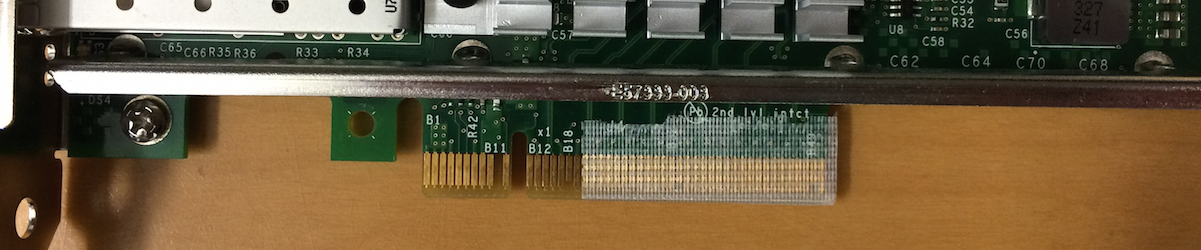
\includegraphics[width=.9\textwidth]{pic/x1.png} \\
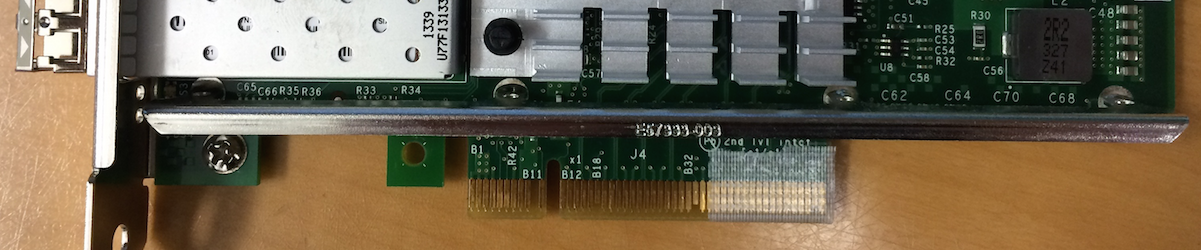
\includegraphics[width=.9\textwidth]{pic/x4.png}

\begin{scriptsize}
\begin{tcolorbox}[width=.9\linewidth]
\$ sudo lspci -vv\\
01:00.0 Ethernet controller: Intel Corporation 82599ES\\
LnkCap: Port \#0, \textbf{Speed 5GT/s, Width x8}, ... \\
LnkSta: \textbf{Speed 5GT/s, Width x1}, ...
\end{tcolorbox}
\end{scriptsize}
\vspace{-.5em}
\small{上: x1マスク, 中: x4マスク, 下: x1時のLink status}
\end{figure}

\end{frame}

%%%%%%%%%%%%%%%%%%%%%%%%


\begin{frame}[fragile,t]{計測環境}

\vspace{-1.5em}
\begin{figure}
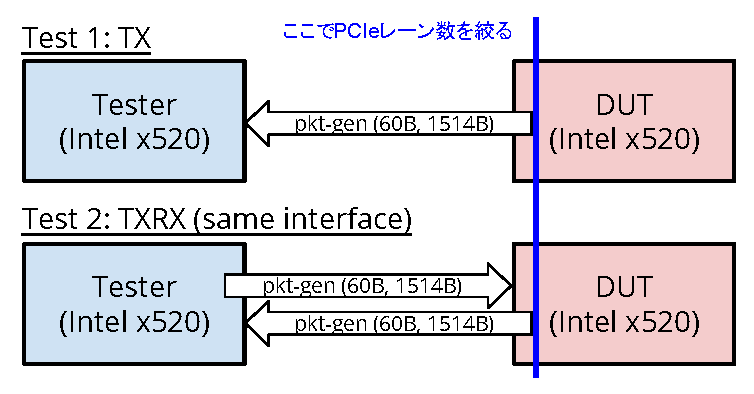
\includegraphics[width=.9\textwidth]{fig/test2.pdf}
\end{figure}

\vspace{-1em}

計測結果の注意点
\vspace{-.5em}
\begin{itemize}
\item Softwareで試験パケットを生成しているので計測PPSに誤差が生じる
\item もちろんx8の時に最大限PCIe性能がだせる回路と考えられるので,NICそのものの絶対評価ではない
\end{itemize}

\end{frame}

%%%%%%%%%%%%%%%%%%%%%%%%%

\begin{frame}{Max. TX Throughput}
	\begin{figure}
		\resizebox{.7\textwidth}{!}{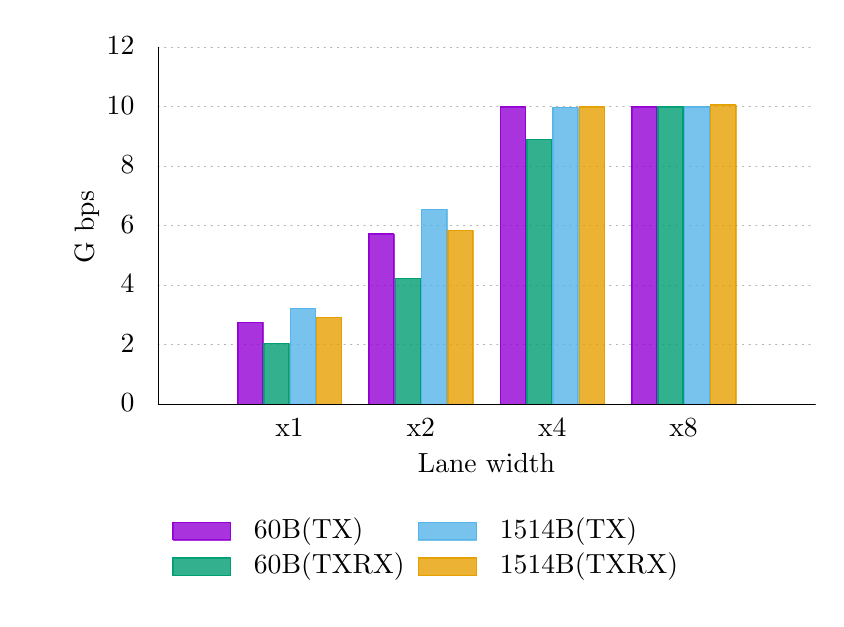
\begin{tikzpicture}[gnuplot]
%% generated with GNUPLOT 5.0p0 (Lua 5.2; terminal rev. 99, script rev. 100)
%% 月  6/29 16:18:40 2015
\path (0.000,0.000) rectangle (10.000,7.000);
\gpcolor{color=gp lt color axes}
\gpsetlinetype{gp lt axes}
\gpsetdashtype{gp dt axes}
\gpsetlinewidth{1.00}
\draw[gp path] (1.656,2.464)--(9.999,2.464);
\gpcolor{color=gp lt color border}
\node[gp node right] at (1.472,2.464) {$0$};
\gpcolor{color=gp lt color axes}
\draw[gp path] (1.656,3.220)--(9.999,3.220);
\gpcolor{color=gp lt color border}
\node[gp node right] at (1.472,3.220) {$2$};
\gpcolor{color=gp lt color axes}
\draw[gp path] (1.656,3.976)--(9.999,3.976);
\gpcolor{color=gp lt color border}
\node[gp node right] at (1.472,3.976) {$4$};
\gpcolor{color=gp lt color axes}
\draw[gp path] (1.656,4.732)--(9.999,4.732);
\gpcolor{color=gp lt color border}
\node[gp node right] at (1.472,4.732) {$6$};
\gpcolor{color=gp lt color axes}
\draw[gp path] (1.656,5.487)--(9.999,5.487);
\gpcolor{color=gp lt color border}
\node[gp node right] at (1.472,5.487) {$8$};
\gpcolor{color=gp lt color axes}
\draw[gp path] (1.656,6.243)--(9.999,6.243);
\gpcolor{color=gp lt color border}
\node[gp node right] at (1.472,6.243) {$10$};
\gpcolor{color=gp lt color axes}
\draw[gp path] (1.656,6.999)--(9.999,6.999);
\gpcolor{color=gp lt color border}
\node[gp node right] at (1.472,6.999) {$12$};
\node[gp node center] at (3.325,2.156) {x1};
\node[gp node center] at (4.993,2.156) {x2};
\node[gp node center] at (6.662,2.156) {x4};
\node[gp node center] at (8.330,2.156) {x8};
\gpsetlinetype{gp lt border}
\gpsetdashtype{gp dt solid}
\draw[gp path] (1.656,6.999)--(1.656,2.464)--(9.999,2.464);
\node[gp node center,rotate=-270] at (0.766,4.731) {G bps};
\node[gp node center] at (5.827,1.694) {Lane width};
\node[gp node left] at (2.756,0.855) {60B(TX)};
\gpfill{rgb color={0.580,0.000,0.827},opacity=0.80} (1.840,0.743)--(2.572,0.743)--(2.572,0.968)--(1.840,0.968)--cycle;
\gpcolor{rgb color={0.580,0.000,0.827}}
\draw[gp path] (1.840,0.743)--(2.572,0.743)--(2.572,0.967)--(1.840,0.967)--cycle;
\gpfill{rgb color={0.580,0.000,0.827},opacity=0.80} (2.666,2.464)--(2.984,2.464)--(2.984,3.511)--(2.666,3.511)--cycle;
\draw[gp path] (2.666,2.464)--(2.666,3.510)--(2.983,3.510)--(2.983,2.464)--cycle;
\gpfill{rgb color={0.580,0.000,0.827},opacity=0.80} (4.334,2.464)--(4.652,2.464)--(4.652,4.633)--(4.334,4.633)--cycle;
\draw[gp path] (4.334,2.464)--(4.334,4.632)--(4.651,4.632)--(4.651,2.464)--cycle;
\gpfill{rgb color={0.580,0.000,0.827},opacity=0.80} (6.003,2.464)--(6.321,2.464)--(6.321,6.244)--(6.003,6.244)--cycle;
\draw[gp path] (6.003,2.464)--(6.003,6.243)--(6.320,6.243)--(6.320,2.464)--cycle;
\gpfill{rgb color={0.580,0.000,0.827},opacity=0.80} (7.671,2.464)--(7.989,2.464)--(7.989,6.244)--(7.671,6.244)--cycle;
\draw[gp path] (7.671,2.464)--(7.671,6.243)--(7.988,6.243)--(7.988,2.464)--cycle;
\gpcolor{color=gp lt color border}
\node[gp node left] at (2.756,0.405) {60B(TXRX)};
\gpfill{rgb color={0.000,0.620,0.451},opacity=0.80} (1.840,0.293)--(2.572,0.293)--(2.572,0.518)--(1.840,0.518)--cycle;
\gpcolor{rgb color={0.000,0.620,0.451}}
\draw[gp path] (1.840,0.293)--(2.572,0.293)--(2.572,0.517)--(1.840,0.517)--cycle;
\gpfill{rgb color={0.000,0.620,0.451},opacity=0.80} (2.999,2.464)--(3.317,2.464)--(3.317,3.238)--(2.999,3.238)--cycle;
\draw[gp path] (2.999,2.464)--(2.999,3.237)--(3.316,3.237)--(3.316,2.464)--cycle;
\gpfill{rgb color={0.000,0.620,0.451},opacity=0.80} (4.668,2.464)--(4.986,2.464)--(4.986,4.069)--(4.668,4.069)--cycle;
\draw[gp path] (4.668,2.464)--(4.668,4.068)--(4.985,4.068)--(4.985,2.464)--cycle;
\gpfill{rgb color={0.000,0.620,0.451},opacity=0.80} (6.336,2.464)--(6.654,2.464)--(6.654,5.833)--(6.336,5.833)--cycle;
\draw[gp path] (6.336,2.464)--(6.336,5.832)--(6.653,5.832)--(6.653,2.464)--cycle;
\gpfill{rgb color={0.000,0.620,0.451},opacity=0.80} (8.005,2.464)--(8.323,2.464)--(8.323,6.244)--(8.005,6.244)--cycle;
\draw[gp path] (8.005,2.464)--(8.005,6.243)--(8.322,6.243)--(8.322,2.464)--cycle;
\gpcolor{color=gp lt color border}
\node[gp node left] at (5.880,0.855) {1514B(TX)};
\gpfill{rgb color={0.337,0.706,0.914},opacity=0.80} (4.964,0.743)--(5.696,0.743)--(5.696,0.968)--(4.964,0.968)--cycle;
\gpcolor{rgb color={0.337,0.706,0.914}}
\draw[gp path] (4.964,0.743)--(5.696,0.743)--(5.696,0.967)--(4.964,0.967)--cycle;
\gpfill{rgb color={0.337,0.706,0.914},opacity=0.80} (3.333,2.464)--(3.651,2.464)--(3.651,3.682)--(3.333,3.682)--cycle;
\draw[gp path] (3.333,2.464)--(3.333,3.681)--(3.650,3.681)--(3.650,2.464)--cycle;
\gpfill{rgb color={0.337,0.706,0.914},opacity=0.80} (5.002,2.464)--(5.320,2.464)--(5.320,4.942)--(5.002,4.942)--cycle;
\draw[gp path] (5.002,2.464)--(5.002,4.941)--(5.319,4.941)--(5.319,2.464)--cycle;
\gpfill{rgb color={0.337,0.706,0.914},opacity=0.80} (6.670,2.464)--(6.988,2.464)--(6.988,6.240)--(6.670,6.240)--cycle;
\draw[gp path] (6.670,2.464)--(6.670,6.239)--(6.987,6.239)--(6.987,2.464)--cycle;
\gpfill{rgb color={0.337,0.706,0.914},opacity=0.80} (8.339,2.464)--(8.657,2.464)--(8.657,6.243)--(8.339,6.243)--cycle;
\draw[gp path] (8.339,2.464)--(8.339,6.242)--(8.656,6.242)--(8.656,2.464)--cycle;
\gpcolor{color=gp lt color border}
\node[gp node left] at (5.880,0.405) {1514B(TXRX)};
\gpfill{rgb color={0.902,0.624,0.000},opacity=0.80} (4.964,0.293)--(5.696,0.293)--(5.696,0.518)--(4.964,0.518)--cycle;
\gpcolor{rgb color={0.902,0.624,0.000}}
\draw[gp path] (4.964,0.293)--(5.696,0.293)--(5.696,0.517)--(4.964,0.517)--cycle;
\gpfill{rgb color={0.902,0.624,0.000},opacity=0.80} (3.667,2.464)--(3.985,2.464)--(3.985,3.569)--(3.667,3.569)--cycle;
\draw[gp path] (3.667,2.464)--(3.667,3.568)--(3.984,3.568)--(3.984,2.464)--cycle;
\gpfill{rgb color={0.902,0.624,0.000},opacity=0.80} (5.335,2.464)--(5.653,2.464)--(5.653,4.679)--(5.335,4.679)--cycle;
\draw[gp path] (5.335,2.464)--(5.335,4.678)--(5.652,4.678)--(5.652,2.464)--cycle;
\gpfill{rgb color={0.902,0.624,0.000},opacity=0.80} (7.004,2.464)--(7.322,2.464)--(7.322,6.245)--(7.004,6.245)--cycle;
\draw[gp path] (7.004,2.464)--(7.004,6.244)--(7.321,6.244)--(7.321,2.464)--cycle;
\gpfill{rgb color={0.902,0.624,0.000},opacity=0.80} (8.672,2.464)--(8.990,2.464)--(8.990,6.269)--(8.672,6.269)--cycle;
\draw[gp path] (8.672,2.464)--(8.672,6.268)--(8.989,6.268)--(8.989,2.464)--cycle;
\gpcolor{color=gp lt color border}
\draw[gp path] (1.656,6.999)--(1.656,2.464)--(9.999,2.464);
%% coordinates of the plot area
\gpdefrectangularnode{gp plot 1}{\pgfpoint{1.656cm}{2.464cm}}{\pgfpoint{9.999cm}{6.999cm}}
\end{tikzpicture}
%% gnuplot variables
}
	\end{figure}
	{\footnotesize Theoretical Max. Throughput (GT/s) * 8b/10b overhead (0.8): \\
	x1: 4Gbps, x2: 8Gbps, x4: 16Gbps, x8: 32Gbps}
\end{frame}

%%%%%%%%%%%%%%%%%%%%%%%%%

\begin{frame}{\% of Max. TX Throughput}
	\begin{figure}
		\resizebox{.7\textwidth}{!}{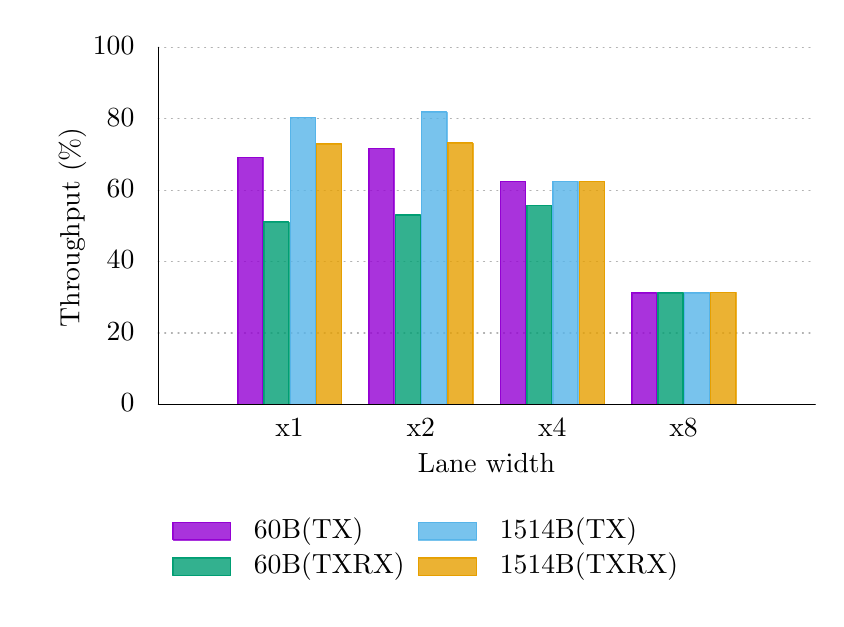
\begin{tikzpicture}[gnuplot]
%% generated with GNUPLOT 5.0p0 (Lua 5.2; terminal rev. 99, script rev. 100)
%% 金  5/ 8 21:37:03 2015
\path (0.000,0.000) rectangle (10.000,7.000);
\gpcolor{color=gp lt color axes}
\gpsetlinetype{gp lt axes}
\gpsetdashtype{gp dt axes}
\gpsetlinewidth{1.00}
\draw[gp path] (1.656,2.464)--(9.999,2.464);
\gpcolor{color=gp lt color border}
\node[gp node right] at (1.472,2.464) {$0$};
\gpcolor{color=gp lt color axes}
\draw[gp path] (1.656,3.371)--(9.999,3.371);
\gpcolor{color=gp lt color border}
\node[gp node right] at (1.472,3.371) {$20$};
\gpcolor{color=gp lt color axes}
\draw[gp path] (1.656,4.278)--(9.999,4.278);
\gpcolor{color=gp lt color border}
\node[gp node right] at (1.472,4.278) {$40$};
\gpcolor{color=gp lt color axes}
\draw[gp path] (1.656,5.185)--(9.999,5.185);
\gpcolor{color=gp lt color border}
\node[gp node right] at (1.472,5.185) {$60$};
\gpcolor{color=gp lt color axes}
\draw[gp path] (1.656,6.092)--(9.999,6.092);
\gpcolor{color=gp lt color border}
\node[gp node right] at (1.472,6.092) {$80$};
\gpcolor{color=gp lt color axes}
\draw[gp path] (1.656,6.999)--(9.999,6.999);
\gpcolor{color=gp lt color border}
\node[gp node right] at (1.472,6.999) {$100$};
\node[gp node center] at (3.325,2.156) {x1};
\node[gp node center] at (4.993,2.156) {x2};
\node[gp node center] at (6.662,2.156) {x4};
\node[gp node center] at (8.330,2.156) {x8};
\gpsetlinetype{gp lt border}
\gpsetdashtype{gp dt solid}
\draw[gp path] (1.656,6.999)--(1.656,2.464)--(9.999,2.464);
\node[gp node center,rotate=-270] at (0.582,4.731) {Throughput (\%)};
\node[gp node center] at (5.827,1.694) {Lane width};
\node[gp node left] at (2.756,0.855) {60B(TX)};
\gpfill{rgb color={0.580,0.000,0.827},opacity=0.80} (1.840,0.743)--(2.572,0.743)--(2.572,0.968)--(1.840,0.968)--cycle;
\gpcolor{rgb color={0.580,0.000,0.827}}
\draw[gp path] (1.840,0.743)--(2.572,0.743)--(2.572,0.967)--(1.840,0.967)--cycle;
\gpfill{rgb color={0.580,0.000,0.827},opacity=0.80} (2.666,2.464)--(2.984,2.464)--(2.984,5.605)--(2.666,5.605)--cycle;
\draw[gp path] (2.666,2.464)--(2.666,5.604)--(2.983,5.604)--(2.983,2.464)--cycle;
\gpfill{rgb color={0.580,0.000,0.827},opacity=0.80} (4.334,2.464)--(4.652,2.464)--(4.652,5.718)--(4.334,5.718)--cycle;
\draw[gp path] (4.334,2.464)--(4.334,5.717)--(4.651,5.717)--(4.651,2.464)--cycle;
\gpfill{rgb color={0.580,0.000,0.827},opacity=0.80} (6.003,2.464)--(6.321,2.464)--(6.321,5.299)--(6.003,5.299)--cycle;
\draw[gp path] (6.003,2.464)--(6.003,5.298)--(6.320,5.298)--(6.320,2.464)--cycle;
\gpfill{rgb color={0.580,0.000,0.827},opacity=0.80} (7.671,2.464)--(7.989,2.464)--(7.989,3.882)--(7.671,3.882)--cycle;
\draw[gp path] (7.671,2.464)--(7.671,3.881)--(7.988,3.881)--(7.988,2.464)--cycle;
\gpcolor{color=gp lt color border}
\node[gp node left] at (2.756,0.405) {60B(TXRX)};
\gpfill{rgb color={0.000,0.620,0.451},opacity=0.80} (1.840,0.293)--(2.572,0.293)--(2.572,0.518)--(1.840,0.518)--cycle;
\gpcolor{rgb color={0.000,0.620,0.451}}
\draw[gp path] (1.840,0.293)--(2.572,0.293)--(2.572,0.517)--(1.840,0.517)--cycle;
\gpfill{rgb color={0.000,0.620,0.451},opacity=0.80} (2.999,2.464)--(3.317,2.464)--(3.317,4.784)--(2.999,4.784)--cycle;
\draw[gp path] (2.999,2.464)--(2.999,4.783)--(3.316,4.783)--(3.316,2.464)--cycle;
\gpfill{rgb color={0.000,0.620,0.451},opacity=0.80} (4.668,2.464)--(4.986,2.464)--(4.986,4.871)--(4.668,4.871)--cycle;
\draw[gp path] (4.668,2.464)--(4.668,4.870)--(4.985,4.870)--(4.985,2.464)--cycle;
\gpfill{rgb color={0.000,0.620,0.451},opacity=0.80} (6.336,2.464)--(6.654,2.464)--(6.654,4.991)--(6.336,4.991)--cycle;
\draw[gp path] (6.336,2.464)--(6.336,4.990)--(6.653,4.990)--(6.653,2.464)--cycle;
\gpfill{rgb color={0.000,0.620,0.451},opacity=0.80} (8.005,2.464)--(8.323,2.464)--(8.323,3.882)--(8.005,3.882)--cycle;
\draw[gp path] (8.005,2.464)--(8.005,3.881)--(8.322,3.881)--(8.322,2.464)--cycle;
\gpcolor{color=gp lt color border}
\node[gp node left] at (5.880,0.855) {1514B(TX)};
\gpfill{rgb color={0.337,0.706,0.914},opacity=0.80} (4.964,0.743)--(5.696,0.743)--(5.696,0.968)--(4.964,0.968)--cycle;
\gpcolor{rgb color={0.337,0.706,0.914}}
\draw[gp path] (4.964,0.743)--(5.696,0.743)--(5.696,0.967)--(4.964,0.967)--cycle;
\gpfill{rgb color={0.337,0.706,0.914},opacity=0.80} (3.333,2.464)--(3.651,2.464)--(3.651,6.114)--(3.333,6.114)--cycle;
\draw[gp path] (3.333,2.464)--(3.333,6.113)--(3.650,6.113)--(3.650,2.464)--cycle;
\gpfill{rgb color={0.337,0.706,0.914},opacity=0.80} (5.002,2.464)--(5.320,2.464)--(5.320,6.181)--(5.002,6.181)--cycle;
\draw[gp path] (5.002,2.464)--(5.002,6.180)--(5.319,6.180)--(5.319,2.464)--cycle;
\gpfill{rgb color={0.337,0.706,0.914},opacity=0.80} (6.670,2.464)--(6.988,2.464)--(6.988,5.296)--(6.670,5.296)--cycle;
\draw[gp path] (6.670,2.464)--(6.670,5.295)--(6.987,5.295)--(6.987,2.464)--cycle;
\gpfill{rgb color={0.337,0.706,0.914},opacity=0.80} (8.339,2.464)--(8.657,2.464)--(8.657,3.882)--(8.339,3.882)--cycle;
\draw[gp path] (8.339,2.464)--(8.339,3.881)--(8.656,3.881)--(8.656,2.464)--cycle;
\gpcolor{color=gp lt color border}
\node[gp node left] at (5.880,0.405) {1514B(TXRX)};
\gpfill{rgb color={0.902,0.624,0.000},opacity=0.80} (4.964,0.293)--(5.696,0.293)--(5.696,0.518)--(4.964,0.518)--cycle;
\gpcolor{rgb color={0.902,0.624,0.000}}
\draw[gp path] (4.964,0.293)--(5.696,0.293)--(5.696,0.517)--(4.964,0.517)--cycle;
\gpfill{rgb color={0.902,0.624,0.000},opacity=0.80} (3.667,2.464)--(3.985,2.464)--(3.985,5.776)--(3.667,5.776)--cycle;
\draw[gp path] (3.667,2.464)--(3.667,5.775)--(3.984,5.775)--(3.984,2.464)--cycle;
\gpfill{rgb color={0.902,0.624,0.000},opacity=0.80} (5.335,2.464)--(5.653,2.464)--(5.653,5.787)--(5.335,5.787)--cycle;
\draw[gp path] (5.335,2.464)--(5.335,5.786)--(5.652,5.786)--(5.652,2.464)--cycle;
\gpfill{rgb color={0.902,0.624,0.000},opacity=0.80} (7.004,2.464)--(7.322,2.464)--(7.322,5.300)--(7.004,5.300)--cycle;
\draw[gp path] (7.004,2.464)--(7.004,5.299)--(7.321,5.299)--(7.321,2.464)--cycle;
\gpfill{rgb color={0.902,0.624,0.000},opacity=0.80} (8.672,2.464)--(8.990,2.464)--(8.990,3.891)--(8.672,3.891)--cycle;
\draw[gp path] (8.672,2.464)--(8.672,3.890)--(8.989,3.890)--(8.989,2.464)--cycle;
\gpcolor{color=gp lt color border}
\draw[gp path] (1.656,6.999)--(1.656,2.464)--(9.999,2.464);
%% coordinates of the plot area
\gpdefrectangularnode{gp plot 1}{\pgfpoint{1.656cm}{2.464cm}}{\pgfpoint{9.999cm}{6.999cm}}
\end{tikzpicture}
%% gnuplot variables
}
	\end{figure}
	{\footnotesize Theoretical Max. Throughput (GT/s) * 8b/10b overhead (0.8): \\
	x1: 4Gbps, x2: 8Gbps, x4: 16Gbps, x8: 32Gbps}
\end{frame}

%%%%%%%%%%%%%%%%%%%%%%%%%

\begin{frame}[fragile,t]{NICのPCIe基礎体力測定 考察}
	\vspace{-2em}
	\begin{figure}
		\resizebox{.8\textwidth}{!}{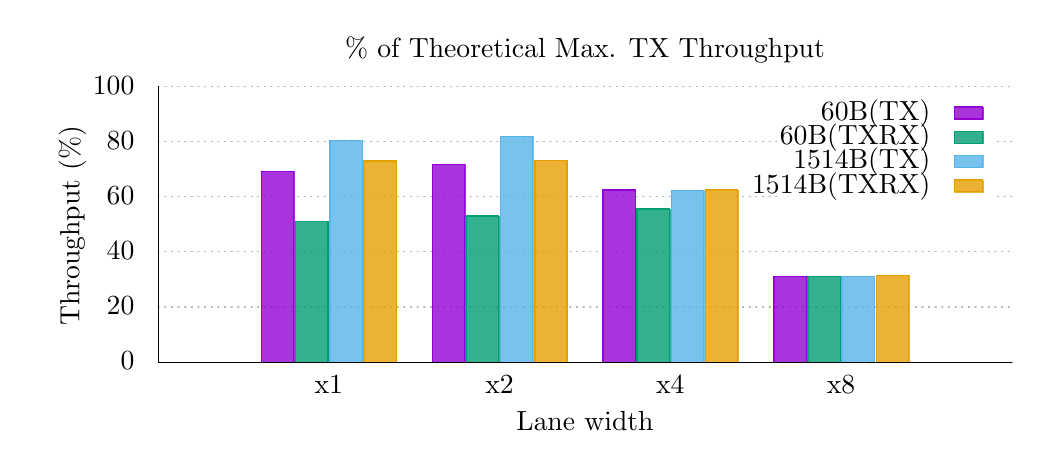
\begin{tikzpicture}[gnuplot]
%% generated with GNUPLOT 5.0p0 (Lua 5.2; terminal rev. 99, script rev. 100)
%% 木  5/ 7 16:28:46 2015
\path (0.000,0.000) rectangle (12.500,3.500);
\gpcolor{color=gp lt color axes}
\gpsetlinetype{gp lt axes}
\gpsetdashtype{gp dt axes}
\gpsetlinewidth{1.00}
\draw[gp path] (1.656,0.000)--(12.499,0.000);
\gpcolor{color=gp lt color border}
\node[gp node right] at (1.472,0.000) {$0$};
\gpcolor{color=gp lt color axes}
\draw[gp path] (1.656,0.700)--(12.499,0.700);
\gpcolor{color=gp lt color border}
\node[gp node right] at (1.472,0.700) {$20$};
\gpcolor{color=gp lt color axes}
\draw[gp path] (1.656,1.400)--(12.499,1.400);
\gpcolor{color=gp lt color border}
\node[gp node right] at (1.472,1.400) {$40$};
\gpcolor{color=gp lt color axes}
\draw[gp path] (1.656,2.099)--(9.559,2.099);
\draw[gp path] (12.315,2.099)--(12.499,2.099);
\gpcolor{color=gp lt color border}
\node[gp node right] at (1.472,2.099) {$60$};
\gpcolor{color=gp lt color axes}
\draw[gp path] (1.656,2.799)--(9.559,2.799);
\draw[gp path] (12.315,2.799)--(12.499,2.799);
\gpcolor{color=gp lt color border}
\node[gp node right] at (1.472,2.799) {$80$};
\gpcolor{color=gp lt color axes}
\draw[gp path] (1.656,3.499)--(12.499,3.499);
\gpcolor{color=gp lt color border}
\node[gp node right] at (1.472,3.499) {$100$};
\node[gp node center] at (3.825,-0.308) {x1};
\node[gp node center] at (5.993,-0.308) {x2};
\node[gp node center] at (8.162,-0.308) {x4};
\node[gp node center] at (10.330,-0.308) {x8};
\gpsetlinetype{gp lt border}
\gpsetdashtype{gp dt solid}
\draw[gp path] (1.656,3.499)--(1.656,0.000)--(12.499,0.000);
\node[gp node center,rotate=-270] at (0.582,1.749) {Throughput (\%)};
\node[gp node center] at (7.077,-0.769) {Lane width};
\node[gp node center] at (7.077,3.961) {\% of Theoretical Max. TX Throughput};
\node[gp node right] at (11.583,3.165) {60B(TX)};
\gpfill{rgb color={0.580,0.000,0.827},opacity=0.80} (11.767,3.088)--(12.131,3.088)--(12.131,3.242)--(11.767,3.242)--cycle;
\gpcolor{rgb color={0.580,0.000,0.827}}
\draw[gp path] (11.767,3.088)--(12.131,3.088)--(12.131,3.242)--(11.767,3.242)--cycle;
\gpfill{rgb color={0.580,0.000,0.827},opacity=0.80} (2.968,0.000)--(3.381,0.000)--(3.381,2.423)--(2.968,2.423)--cycle;
\draw[gp path] (2.968,0.000)--(2.968,2.422)--(3.380,2.422)--(3.380,0.000)--cycle;
\gpfill{rgb color={0.580,0.000,0.827},opacity=0.80} (5.137,0.000)--(5.550,0.000)--(5.550,2.510)--(5.137,2.510)--cycle;
\draw[gp path] (5.137,0.000)--(5.137,2.509)--(5.549,2.509)--(5.549,0.000)--cycle;
\gpfill{rgb color={0.580,0.000,0.827},opacity=0.80} (7.305,0.000)--(7.718,0.000)--(7.718,2.188)--(7.305,2.188)--cycle;
\draw[gp path] (7.305,0.000)--(7.305,2.187)--(7.717,2.187)--(7.717,0.000)--cycle;
\gpfill{rgb color={0.580,0.000,0.827},opacity=0.80} (9.474,0.000)--(9.887,0.000)--(9.887,1.094)--(9.474,1.094)--cycle;
\draw[gp path] (9.474,0.000)--(9.474,1.093)--(9.886,1.093)--(9.886,0.000)--cycle;
\gpcolor{color=gp lt color border}
\node[gp node right] at (11.583,2.857) {60B(TXRX)};
\gpfill{rgb color={0.000,0.620,0.451},opacity=0.80} (11.767,2.780)--(12.131,2.780)--(12.131,2.934)--(11.767,2.934)--cycle;
\gpcolor{rgb color={0.000,0.620,0.451}}
\draw[gp path] (11.767,2.780)--(12.131,2.780)--(12.131,2.934)--(11.767,2.934)--cycle;
\gpfill{rgb color={0.000,0.620,0.451},opacity=0.80} (3.402,0.000)--(3.815,0.000)--(3.815,1.790)--(3.402,1.790)--cycle;
\draw[gp path] (3.402,0.000)--(3.402,1.789)--(3.814,1.789)--(3.814,0.000)--cycle;
\gpfill{rgb color={0.000,0.620,0.451},opacity=0.80} (5.570,0.000)--(5.983,0.000)--(5.983,1.857)--(5.570,1.857)--cycle;
\draw[gp path] (5.570,0.000)--(5.570,1.856)--(5.982,1.856)--(5.982,0.000)--cycle;
\gpfill{rgb color={0.000,0.620,0.451},opacity=0.80} (7.739,0.000)--(8.152,0.000)--(8.152,1.950)--(7.739,1.950)--cycle;
\draw[gp path] (7.739,0.000)--(7.739,1.949)--(8.151,1.949)--(8.151,0.000)--cycle;
\gpfill{rgb color={0.000,0.620,0.451},opacity=0.80} (9.908,0.000)--(10.321,0.000)--(10.321,1.094)--(9.908,1.094)--cycle;
\draw[gp path] (9.908,0.000)--(9.908,1.093)--(10.320,1.093)--(10.320,0.000)--cycle;
\gpcolor{color=gp lt color border}
\node[gp node right] at (11.583,2.549) {1514B(TX)};
\gpfill{rgb color={0.337,0.706,0.914},opacity=0.80} (11.767,2.472)--(12.131,2.472)--(12.131,2.626)--(11.767,2.626)--cycle;
\gpcolor{rgb color={0.337,0.706,0.914}}
\draw[gp path] (11.767,2.472)--(12.131,2.472)--(12.131,2.626)--(11.767,2.626)--cycle;
\gpfill{rgb color={0.337,0.706,0.914},opacity=0.80} (3.835,0.000)--(4.248,0.000)--(4.248,2.817)--(3.835,2.817)--cycle;
\draw[gp path] (3.835,0.000)--(3.835,2.816)--(4.247,2.816)--(4.247,0.000)--cycle;
\gpfill{rgb color={0.337,0.706,0.914},opacity=0.80} (6.004,0.000)--(6.417,0.000)--(6.417,2.868)--(6.004,2.868)--cycle;
\draw[gp path] (6.004,0.000)--(6.004,2.867)--(6.416,2.867)--(6.416,0.000)--cycle;
\gpfill{rgb color={0.337,0.706,0.914},opacity=0.80} (8.173,0.000)--(8.586,0.000)--(8.586,2.185)--(8.173,2.185)--cycle;
\draw[gp path] (8.173,0.000)--(8.173,2.184)--(8.585,2.184)--(8.585,0.000)--cycle;
\gpfill{rgb color={0.337,0.706,0.914},opacity=0.80} (10.341,0.000)--(10.754,0.000)--(10.754,1.094)--(10.341,1.094)--cycle;
\draw[gp path] (10.341,0.000)--(10.341,1.093)--(10.753,1.093)--(10.753,0.000)--cycle;
\gpcolor{color=gp lt color border}
\node[gp node right] at (11.583,2.241) {1514B(TXRX)};
\gpfill{rgb color={0.902,0.624,0.000},opacity=0.80} (11.767,2.164)--(12.131,2.164)--(12.131,2.318)--(11.767,2.318)--cycle;
\gpcolor{rgb color={0.902,0.624,0.000}}
\draw[gp path] (11.767,2.164)--(12.131,2.164)--(12.131,2.318)--(11.767,2.318)--cycle;
\gpfill{rgb color={0.902,0.624,0.000},opacity=0.80} (4.269,0.000)--(4.682,0.000)--(4.682,2.555)--(4.269,2.555)--cycle;
\draw[gp path] (4.269,0.000)--(4.269,2.554)--(4.681,2.554)--(4.681,0.000)--cycle;
\gpfill{rgb color={0.902,0.624,0.000},opacity=0.80} (6.438,0.000)--(6.851,0.000)--(6.851,2.564)--(6.438,2.564)--cycle;
\draw[gp path] (6.438,0.000)--(6.438,2.563)--(6.850,2.563)--(6.850,0.000)--cycle;
\gpfill{rgb color={0.902,0.624,0.000},opacity=0.80} (8.606,0.000)--(9.019,0.000)--(9.019,2.189)--(8.606,2.189)--cycle;
\draw[gp path] (8.606,0.000)--(8.606,2.188)--(9.018,2.188)--(9.018,0.000)--cycle;
\gpfill{rgb color={0.902,0.624,0.000},opacity=0.80} (10.775,0.000)--(11.188,0.000)--(11.188,1.101)--(10.775,1.101)--cycle;
\draw[gp path] (10.775,0.000)--(10.775,1.100)--(11.187,1.100)--(11.187,0.000)--cycle;
\gpcolor{color=gp lt color border}
\draw[gp path] (1.656,3.499)--(1.656,0.000)--(12.499,0.000);
%% coordinates of the plot area
\gpdefrectangularnode{gp plot 1}{\pgfpoint{1.656cm}{0.000cm}}{\pgfpoint{12.499cm}{3.499cm}}
\end{tikzpicture}
%% gnuplot variables
}
	\end{figure}
	\vspace{-1.5em}

	PCIe利用可能帯域を計測することでNIC回路の性能を推測
	\vspace{-.5em}
	\begin{itemize}
		\item 送信のみの場合,PCIeの約81\%の帯域が利用可能
		\item 送受信時,PCIeの約73\%の帯域が利用可能
		\item 送受信時,1514B-60Bで約20\%利用可能帯域が減少
		\item (PCIeはFull duplexにも関わらず) 60B送受信-送信のみ \\
		      で,PCIe利用可能帯域が約18\%減少
	\end{itemize}
\end{frame}

%%%%%%%%%%%%%%%%%%%%%%%%%

\begin{frame}[fragile,t]{NICのPCIe基礎体力測定 考察}
	\vspace{-2em}
	\begin{figure}
		\resizebox{.8\textwidth}{!}{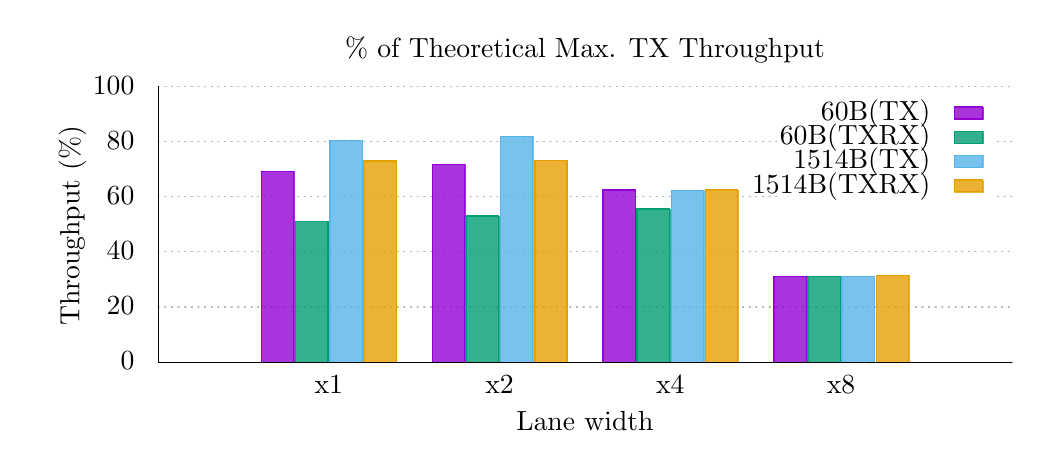
\begin{tikzpicture}[gnuplot]
%% generated with GNUPLOT 5.0p0 (Lua 5.2; terminal rev. 99, script rev. 100)
%% 木  5/ 7 16:28:46 2015
\path (0.000,0.000) rectangle (12.500,3.500);
\gpcolor{color=gp lt color axes}
\gpsetlinetype{gp lt axes}
\gpsetdashtype{gp dt axes}
\gpsetlinewidth{1.00}
\draw[gp path] (1.656,0.000)--(12.499,0.000);
\gpcolor{color=gp lt color border}
\node[gp node right] at (1.472,0.000) {$0$};
\gpcolor{color=gp lt color axes}
\draw[gp path] (1.656,0.700)--(12.499,0.700);
\gpcolor{color=gp lt color border}
\node[gp node right] at (1.472,0.700) {$20$};
\gpcolor{color=gp lt color axes}
\draw[gp path] (1.656,1.400)--(12.499,1.400);
\gpcolor{color=gp lt color border}
\node[gp node right] at (1.472,1.400) {$40$};
\gpcolor{color=gp lt color axes}
\draw[gp path] (1.656,2.099)--(9.559,2.099);
\draw[gp path] (12.315,2.099)--(12.499,2.099);
\gpcolor{color=gp lt color border}
\node[gp node right] at (1.472,2.099) {$60$};
\gpcolor{color=gp lt color axes}
\draw[gp path] (1.656,2.799)--(9.559,2.799);
\draw[gp path] (12.315,2.799)--(12.499,2.799);
\gpcolor{color=gp lt color border}
\node[gp node right] at (1.472,2.799) {$80$};
\gpcolor{color=gp lt color axes}
\draw[gp path] (1.656,3.499)--(12.499,3.499);
\gpcolor{color=gp lt color border}
\node[gp node right] at (1.472,3.499) {$100$};
\node[gp node center] at (3.825,-0.308) {x1};
\node[gp node center] at (5.993,-0.308) {x2};
\node[gp node center] at (8.162,-0.308) {x4};
\node[gp node center] at (10.330,-0.308) {x8};
\gpsetlinetype{gp lt border}
\gpsetdashtype{gp dt solid}
\draw[gp path] (1.656,3.499)--(1.656,0.000)--(12.499,0.000);
\node[gp node center,rotate=-270] at (0.582,1.749) {Throughput (\%)};
\node[gp node center] at (7.077,-0.769) {Lane width};
\node[gp node center] at (7.077,3.961) {\% of Theoretical Max. TX Throughput};
\node[gp node right] at (11.583,3.165) {60B(TX)};
\gpfill{rgb color={0.580,0.000,0.827},opacity=0.80} (11.767,3.088)--(12.131,3.088)--(12.131,3.242)--(11.767,3.242)--cycle;
\gpcolor{rgb color={0.580,0.000,0.827}}
\draw[gp path] (11.767,3.088)--(12.131,3.088)--(12.131,3.242)--(11.767,3.242)--cycle;
\gpfill{rgb color={0.580,0.000,0.827},opacity=0.80} (2.968,0.000)--(3.381,0.000)--(3.381,2.423)--(2.968,2.423)--cycle;
\draw[gp path] (2.968,0.000)--(2.968,2.422)--(3.380,2.422)--(3.380,0.000)--cycle;
\gpfill{rgb color={0.580,0.000,0.827},opacity=0.80} (5.137,0.000)--(5.550,0.000)--(5.550,2.510)--(5.137,2.510)--cycle;
\draw[gp path] (5.137,0.000)--(5.137,2.509)--(5.549,2.509)--(5.549,0.000)--cycle;
\gpfill{rgb color={0.580,0.000,0.827},opacity=0.80} (7.305,0.000)--(7.718,0.000)--(7.718,2.188)--(7.305,2.188)--cycle;
\draw[gp path] (7.305,0.000)--(7.305,2.187)--(7.717,2.187)--(7.717,0.000)--cycle;
\gpfill{rgb color={0.580,0.000,0.827},opacity=0.80} (9.474,0.000)--(9.887,0.000)--(9.887,1.094)--(9.474,1.094)--cycle;
\draw[gp path] (9.474,0.000)--(9.474,1.093)--(9.886,1.093)--(9.886,0.000)--cycle;
\gpcolor{color=gp lt color border}
\node[gp node right] at (11.583,2.857) {60B(TXRX)};
\gpfill{rgb color={0.000,0.620,0.451},opacity=0.80} (11.767,2.780)--(12.131,2.780)--(12.131,2.934)--(11.767,2.934)--cycle;
\gpcolor{rgb color={0.000,0.620,0.451}}
\draw[gp path] (11.767,2.780)--(12.131,2.780)--(12.131,2.934)--(11.767,2.934)--cycle;
\gpfill{rgb color={0.000,0.620,0.451},opacity=0.80} (3.402,0.000)--(3.815,0.000)--(3.815,1.790)--(3.402,1.790)--cycle;
\draw[gp path] (3.402,0.000)--(3.402,1.789)--(3.814,1.789)--(3.814,0.000)--cycle;
\gpfill{rgb color={0.000,0.620,0.451},opacity=0.80} (5.570,0.000)--(5.983,0.000)--(5.983,1.857)--(5.570,1.857)--cycle;
\draw[gp path] (5.570,0.000)--(5.570,1.856)--(5.982,1.856)--(5.982,0.000)--cycle;
\gpfill{rgb color={0.000,0.620,0.451},opacity=0.80} (7.739,0.000)--(8.152,0.000)--(8.152,1.950)--(7.739,1.950)--cycle;
\draw[gp path] (7.739,0.000)--(7.739,1.949)--(8.151,1.949)--(8.151,0.000)--cycle;
\gpfill{rgb color={0.000,0.620,0.451},opacity=0.80} (9.908,0.000)--(10.321,0.000)--(10.321,1.094)--(9.908,1.094)--cycle;
\draw[gp path] (9.908,0.000)--(9.908,1.093)--(10.320,1.093)--(10.320,0.000)--cycle;
\gpcolor{color=gp lt color border}
\node[gp node right] at (11.583,2.549) {1514B(TX)};
\gpfill{rgb color={0.337,0.706,0.914},opacity=0.80} (11.767,2.472)--(12.131,2.472)--(12.131,2.626)--(11.767,2.626)--cycle;
\gpcolor{rgb color={0.337,0.706,0.914}}
\draw[gp path] (11.767,2.472)--(12.131,2.472)--(12.131,2.626)--(11.767,2.626)--cycle;
\gpfill{rgb color={0.337,0.706,0.914},opacity=0.80} (3.835,0.000)--(4.248,0.000)--(4.248,2.817)--(3.835,2.817)--cycle;
\draw[gp path] (3.835,0.000)--(3.835,2.816)--(4.247,2.816)--(4.247,0.000)--cycle;
\gpfill{rgb color={0.337,0.706,0.914},opacity=0.80} (6.004,0.000)--(6.417,0.000)--(6.417,2.868)--(6.004,2.868)--cycle;
\draw[gp path] (6.004,0.000)--(6.004,2.867)--(6.416,2.867)--(6.416,0.000)--cycle;
\gpfill{rgb color={0.337,0.706,0.914},opacity=0.80} (8.173,0.000)--(8.586,0.000)--(8.586,2.185)--(8.173,2.185)--cycle;
\draw[gp path] (8.173,0.000)--(8.173,2.184)--(8.585,2.184)--(8.585,0.000)--cycle;
\gpfill{rgb color={0.337,0.706,0.914},opacity=0.80} (10.341,0.000)--(10.754,0.000)--(10.754,1.094)--(10.341,1.094)--cycle;
\draw[gp path] (10.341,0.000)--(10.341,1.093)--(10.753,1.093)--(10.753,0.000)--cycle;
\gpcolor{color=gp lt color border}
\node[gp node right] at (11.583,2.241) {1514B(TXRX)};
\gpfill{rgb color={0.902,0.624,0.000},opacity=0.80} (11.767,2.164)--(12.131,2.164)--(12.131,2.318)--(11.767,2.318)--cycle;
\gpcolor{rgb color={0.902,0.624,0.000}}
\draw[gp path] (11.767,2.164)--(12.131,2.164)--(12.131,2.318)--(11.767,2.318)--cycle;
\gpfill{rgb color={0.902,0.624,0.000},opacity=0.80} (4.269,0.000)--(4.682,0.000)--(4.682,2.555)--(4.269,2.555)--cycle;
\draw[gp path] (4.269,0.000)--(4.269,2.554)--(4.681,2.554)--(4.681,0.000)--cycle;
\gpfill{rgb color={0.902,0.624,0.000},opacity=0.80} (6.438,0.000)--(6.851,0.000)--(6.851,2.564)--(6.438,2.564)--cycle;
\draw[gp path] (6.438,0.000)--(6.438,2.563)--(6.850,2.563)--(6.850,0.000)--cycle;
\gpfill{rgb color={0.902,0.624,0.000},opacity=0.80} (8.606,0.000)--(9.019,0.000)--(9.019,2.189)--(8.606,2.189)--cycle;
\draw[gp path] (8.606,0.000)--(8.606,2.188)--(9.018,2.188)--(9.018,0.000)--cycle;
\gpfill{rgb color={0.902,0.624,0.000},opacity=0.80} (10.775,0.000)--(11.188,0.000)--(11.188,1.101)--(10.775,1.101)--cycle;
\draw[gp path] (10.775,0.000)--(10.775,1.100)--(11.187,1.100)--(11.187,0.000)--cycle;
\gpcolor{color=gp lt color border}
\draw[gp path] (1.656,3.499)--(1.656,0.000)--(12.499,0.000);
%% coordinates of the plot area
\gpdefrectangularnode{gp plot 1}{\pgfpoint{1.656cm}{0.000cm}}{\pgfpoint{12.499cm}{3.499cm}}
\end{tikzpicture}
%% gnuplot variables
}
	\end{figure}
	\vspace{-1.5em}

	\begin{itemize}
		\item PCIeの最大利用可能帯域の割合で見るとx1, x2で同じ傾向
		\item x4(TXRX60B以外)とx8では,Ethernet帯域(10Gbps)を上回るので特性は見えない
	\end{itemize}

	\hspace{-0.5em}検討内容
	\vspace{-.5em}
	\begin{enumerate}
		\item パケットサイズとPCIe利用可能帯域の関係
		\item Full duplexとPCIe利用可能帯域の関係
	\end{enumerate}
\end{frame}

%%%%%%%%%%%%%%%%%%%%%%%%%

\begin{frame}[fragile,t]{NICのおさらい}

\hspace{-0.5em}
\textcolor{blue}{パケット送信時のPCIe操作}
\vspace{-.5em}
\begin{enumerate}
	\item ドライバがNICのリングバッファのTail pointerを更新
	\item データ転送 (DMA read)
	\item Write-back the NIC status
\end{enumerate}

\hspace{-0.5em}
\textcolor{blue}{パケット受信時のPCIe操作}
\vspace{-.5em}
\begin{enumerate}
	\item データ転送 (DMA write)
	\item ドライバがTail pointerを更新
\end{enumerate}
\end{frame}

%%%%%%%%%%%%%%%%%%%%%%%%%

\begin{frame}[fragile,t]{PCIeのおさらい}

\begin{itemize}
	\item PCIeのメモリ操作は送受信のレーンを使ってTLPパケットの通信が発生
	\item Ethernetポートを送受信パケットでFull duplex専有しても,PCIeでは上り下りリンクの専有ができるわけではない ⇛ TLPパケットの送信待ちが発生する
\end{itemize}

\hspace{-0.5em}
\textcolor{blue}{Ethernetパケット送信 (DMA read)}
\vspace{-.5em}
\begin{enumerate}
	\item TLP (Memory read)を送信
	\item ACKとデータ付きコンプリーションを受信
	\item コンプリーションに対するACKを送信
\end{enumerate}

\hspace{-0.5em}
\textcolor{blue}{Ethernetパケット受信時 (DMA write)}
\vspace{-.5em}
\begin{enumerate}
	\item TLP (Memory write)を送信
	\item ACKを受信
\end{enumerate}
\end{frame}

%%%%%%%%%%%%%%%%%%%%%%%%%

\begin{frame}[fragile,t]{計測結果をどう考えるか}
	\vspace{-2em}
	\begin{figure}
		\resizebox{.8\textwidth}{!}{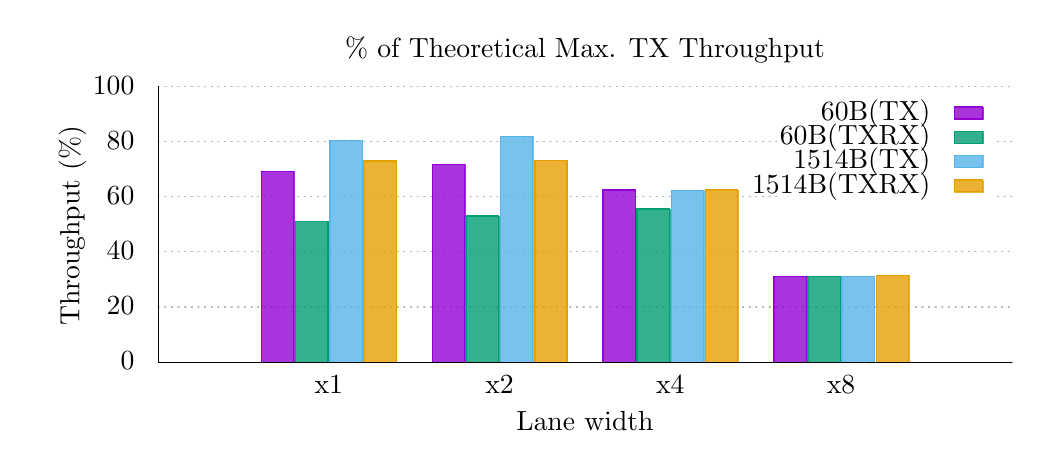
\begin{tikzpicture}[gnuplot]
%% generated with GNUPLOT 5.0p0 (Lua 5.2; terminal rev. 99, script rev. 100)
%% 木  5/ 7 16:28:46 2015
\path (0.000,0.000) rectangle (12.500,3.500);
\gpcolor{color=gp lt color axes}
\gpsetlinetype{gp lt axes}
\gpsetdashtype{gp dt axes}
\gpsetlinewidth{1.00}
\draw[gp path] (1.656,0.000)--(12.499,0.000);
\gpcolor{color=gp lt color border}
\node[gp node right] at (1.472,0.000) {$0$};
\gpcolor{color=gp lt color axes}
\draw[gp path] (1.656,0.700)--(12.499,0.700);
\gpcolor{color=gp lt color border}
\node[gp node right] at (1.472,0.700) {$20$};
\gpcolor{color=gp lt color axes}
\draw[gp path] (1.656,1.400)--(12.499,1.400);
\gpcolor{color=gp lt color border}
\node[gp node right] at (1.472,1.400) {$40$};
\gpcolor{color=gp lt color axes}
\draw[gp path] (1.656,2.099)--(9.559,2.099);
\draw[gp path] (12.315,2.099)--(12.499,2.099);
\gpcolor{color=gp lt color border}
\node[gp node right] at (1.472,2.099) {$60$};
\gpcolor{color=gp lt color axes}
\draw[gp path] (1.656,2.799)--(9.559,2.799);
\draw[gp path] (12.315,2.799)--(12.499,2.799);
\gpcolor{color=gp lt color border}
\node[gp node right] at (1.472,2.799) {$80$};
\gpcolor{color=gp lt color axes}
\draw[gp path] (1.656,3.499)--(12.499,3.499);
\gpcolor{color=gp lt color border}
\node[gp node right] at (1.472,3.499) {$100$};
\node[gp node center] at (3.825,-0.308) {x1};
\node[gp node center] at (5.993,-0.308) {x2};
\node[gp node center] at (8.162,-0.308) {x4};
\node[gp node center] at (10.330,-0.308) {x8};
\gpsetlinetype{gp lt border}
\gpsetdashtype{gp dt solid}
\draw[gp path] (1.656,3.499)--(1.656,0.000)--(12.499,0.000);
\node[gp node center,rotate=-270] at (0.582,1.749) {Throughput (\%)};
\node[gp node center] at (7.077,-0.769) {Lane width};
\node[gp node center] at (7.077,3.961) {\% of Theoretical Max. TX Throughput};
\node[gp node right] at (11.583,3.165) {60B(TX)};
\gpfill{rgb color={0.580,0.000,0.827},opacity=0.80} (11.767,3.088)--(12.131,3.088)--(12.131,3.242)--(11.767,3.242)--cycle;
\gpcolor{rgb color={0.580,0.000,0.827}}
\draw[gp path] (11.767,3.088)--(12.131,3.088)--(12.131,3.242)--(11.767,3.242)--cycle;
\gpfill{rgb color={0.580,0.000,0.827},opacity=0.80} (2.968,0.000)--(3.381,0.000)--(3.381,2.423)--(2.968,2.423)--cycle;
\draw[gp path] (2.968,0.000)--(2.968,2.422)--(3.380,2.422)--(3.380,0.000)--cycle;
\gpfill{rgb color={0.580,0.000,0.827},opacity=0.80} (5.137,0.000)--(5.550,0.000)--(5.550,2.510)--(5.137,2.510)--cycle;
\draw[gp path] (5.137,0.000)--(5.137,2.509)--(5.549,2.509)--(5.549,0.000)--cycle;
\gpfill{rgb color={0.580,0.000,0.827},opacity=0.80} (7.305,0.000)--(7.718,0.000)--(7.718,2.188)--(7.305,2.188)--cycle;
\draw[gp path] (7.305,0.000)--(7.305,2.187)--(7.717,2.187)--(7.717,0.000)--cycle;
\gpfill{rgb color={0.580,0.000,0.827},opacity=0.80} (9.474,0.000)--(9.887,0.000)--(9.887,1.094)--(9.474,1.094)--cycle;
\draw[gp path] (9.474,0.000)--(9.474,1.093)--(9.886,1.093)--(9.886,0.000)--cycle;
\gpcolor{color=gp lt color border}
\node[gp node right] at (11.583,2.857) {60B(TXRX)};
\gpfill{rgb color={0.000,0.620,0.451},opacity=0.80} (11.767,2.780)--(12.131,2.780)--(12.131,2.934)--(11.767,2.934)--cycle;
\gpcolor{rgb color={0.000,0.620,0.451}}
\draw[gp path] (11.767,2.780)--(12.131,2.780)--(12.131,2.934)--(11.767,2.934)--cycle;
\gpfill{rgb color={0.000,0.620,0.451},opacity=0.80} (3.402,0.000)--(3.815,0.000)--(3.815,1.790)--(3.402,1.790)--cycle;
\draw[gp path] (3.402,0.000)--(3.402,1.789)--(3.814,1.789)--(3.814,0.000)--cycle;
\gpfill{rgb color={0.000,0.620,0.451},opacity=0.80} (5.570,0.000)--(5.983,0.000)--(5.983,1.857)--(5.570,1.857)--cycle;
\draw[gp path] (5.570,0.000)--(5.570,1.856)--(5.982,1.856)--(5.982,0.000)--cycle;
\gpfill{rgb color={0.000,0.620,0.451},opacity=0.80} (7.739,0.000)--(8.152,0.000)--(8.152,1.950)--(7.739,1.950)--cycle;
\draw[gp path] (7.739,0.000)--(7.739,1.949)--(8.151,1.949)--(8.151,0.000)--cycle;
\gpfill{rgb color={0.000,0.620,0.451},opacity=0.80} (9.908,0.000)--(10.321,0.000)--(10.321,1.094)--(9.908,1.094)--cycle;
\draw[gp path] (9.908,0.000)--(9.908,1.093)--(10.320,1.093)--(10.320,0.000)--cycle;
\gpcolor{color=gp lt color border}
\node[gp node right] at (11.583,2.549) {1514B(TX)};
\gpfill{rgb color={0.337,0.706,0.914},opacity=0.80} (11.767,2.472)--(12.131,2.472)--(12.131,2.626)--(11.767,2.626)--cycle;
\gpcolor{rgb color={0.337,0.706,0.914}}
\draw[gp path] (11.767,2.472)--(12.131,2.472)--(12.131,2.626)--(11.767,2.626)--cycle;
\gpfill{rgb color={0.337,0.706,0.914},opacity=0.80} (3.835,0.000)--(4.248,0.000)--(4.248,2.817)--(3.835,2.817)--cycle;
\draw[gp path] (3.835,0.000)--(3.835,2.816)--(4.247,2.816)--(4.247,0.000)--cycle;
\gpfill{rgb color={0.337,0.706,0.914},opacity=0.80} (6.004,0.000)--(6.417,0.000)--(6.417,2.868)--(6.004,2.868)--cycle;
\draw[gp path] (6.004,0.000)--(6.004,2.867)--(6.416,2.867)--(6.416,0.000)--cycle;
\gpfill{rgb color={0.337,0.706,0.914},opacity=0.80} (8.173,0.000)--(8.586,0.000)--(8.586,2.185)--(8.173,2.185)--cycle;
\draw[gp path] (8.173,0.000)--(8.173,2.184)--(8.585,2.184)--(8.585,0.000)--cycle;
\gpfill{rgb color={0.337,0.706,0.914},opacity=0.80} (10.341,0.000)--(10.754,0.000)--(10.754,1.094)--(10.341,1.094)--cycle;
\draw[gp path] (10.341,0.000)--(10.341,1.093)--(10.753,1.093)--(10.753,0.000)--cycle;
\gpcolor{color=gp lt color border}
\node[gp node right] at (11.583,2.241) {1514B(TXRX)};
\gpfill{rgb color={0.902,0.624,0.000},opacity=0.80} (11.767,2.164)--(12.131,2.164)--(12.131,2.318)--(11.767,2.318)--cycle;
\gpcolor{rgb color={0.902,0.624,0.000}}
\draw[gp path] (11.767,2.164)--(12.131,2.164)--(12.131,2.318)--(11.767,2.318)--cycle;
\gpfill{rgb color={0.902,0.624,0.000},opacity=0.80} (4.269,0.000)--(4.682,0.000)--(4.682,2.555)--(4.269,2.555)--cycle;
\draw[gp path] (4.269,0.000)--(4.269,2.554)--(4.681,2.554)--(4.681,0.000)--cycle;
\gpfill{rgb color={0.902,0.624,0.000},opacity=0.80} (6.438,0.000)--(6.851,0.000)--(6.851,2.564)--(6.438,2.564)--cycle;
\draw[gp path] (6.438,0.000)--(6.438,2.563)--(6.850,2.563)--(6.850,0.000)--cycle;
\gpfill{rgb color={0.902,0.624,0.000},opacity=0.80} (8.606,0.000)--(9.019,0.000)--(9.019,2.189)--(8.606,2.189)--cycle;
\draw[gp path] (8.606,0.000)--(8.606,2.188)--(9.018,2.188)--(9.018,0.000)--cycle;
\gpfill{rgb color={0.902,0.624,0.000},opacity=0.80} (10.775,0.000)--(11.188,0.000)--(11.188,1.101)--(10.775,1.101)--cycle;
\draw[gp path] (10.775,0.000)--(10.775,1.100)--(11.187,1.100)--(11.187,0.000)--cycle;
\gpcolor{color=gp lt color border}
\draw[gp path] (1.656,3.499)--(1.656,0.000)--(12.499,0.000);
%% coordinates of the plot area
\gpdefrectangularnode{gp plot 1}{\pgfpoint{1.656cm}{0.000cm}}{\pgfpoint{12.499cm}{3.499cm}}
\end{tikzpicture}
%% gnuplot variables
}
	\end{figure}
	\vspace{-2em}

	\begin{table}
	\small{参考データ}
	\begin{tabular}{l|l|l|l}
		\toprule
		  & Throughput & \%. gen3x8(64Gbps) & \%. gen3x16(128Gbps) \\
		\midrule
		10GE & 10Gbps & 15  & 8 \\
		40GE & 40Gbps & 62  & 31 \\
		100GE & 100Gbps & - & 78 \\
		\bottomrule
	\end{tabular}
	\end{table}

	\small{Xeon環境があるとPCMでもう少し詳細がわかりそう}

	\small{NICのレーン数の変更はEEPROMの書き換えで変更できるかも}

\end{frame}

%%%%%%%%%%%%%%%%%%%%%%%%%

\plain{ざっくばらんにFPGA開発ネタ}

%%%%%%%%%%%%%%%%%%%%%%%%%

\begin{frame}[fragile,t]{FPGA開発環境の話}
\begin{itemize}
	\item Xilinx vivadoではSystemverilogで論理合成が可能になった
	\vspace{-0.7em}
	\begin{itemize}
		\item 使える型が増えた (typedef, union, struct, enum, etc) \\
		      ⇛ FPGA回路の合成時に型のチェックができるだけでもかなりうれしい
		\item Classなど合成できないSVの機能はまだまだ多い
		\item FPGAでのunionやenumはとても強力
		\item VHDL, Verilog混在環境で合成可能
	\end{itemize}
	\item Systemverilogがとても良かったので合成可能なパケット処理を考えてみる
	\begin{itemize}
		\item Classなどが使えないのでOSSで公開されているような検証用ライブラリはそのままでは使えない
		\item そこでLinuxのRaw socketぽくしてみる
	\end{itemize}
\end{itemize}
\end{frame}

%%%%%%%%%%%%%%%%%%%%%%%%%

\begin{frame}[fragile,t]
  \frametitle{Systemverilogによるパケット処理 [1/3]}

\begin{figure}
\begin{tcolorbox}[title=ethernet\_pkg.sv]
\begin{minted}[fontsize=\small]{verilog}
/* MAC adderss */
typedef bit [ETH_ALEN-1:0][7:0] macaddr_t;

/* ethernet header */
typedef struct packed {
    macaddr_t h_dest;
    macaddr_t h_source;
    bit [15:0] h_proto;
} ethhdr;
\end{minted}
\end{tcolorbox}
\end{figure}

\end{frame}

%%%%%%%%%%%%%%%%%%%%%%%

\begin{frame}[fragile,t]
  \frametitle{Systemverilogによるパケット処理 [2/3]}

\begin{figure}
\begin{tcolorbox}[title=user\_app.sv]
\begin{minted}[fontsize=\small]{verilog}
union packed {
    bit [5:0][63:0] raw;      // XGMII (64bit)
    struct packed {
        ethhdr eth;
        iphdr ip;
        udphdr udp;
        bit [47:0] padding;
    } hdr;
} tx_pkt, rx_pkt;
\end{minted}
\end{tcolorbox}
\end{figure}

\end{frame}

%%%%%%%%%%%%%%%%%%%%%%%%%


\begin{frame}[fragile,t]
  \frametitle{Systemverilogによるパケット処理 [3/3]}

\vspace{-1em}

\begin{figure}
\begin{tcolorbox}[title=TX]
\begin{minted}[fontsize=\small]{verilog}
// User register to XGMII_TX
xgmii.data = endian_conv64(tx_pkt.raw[5]);
\end{minted}
\end{tcolorbox}
%
\begin{tcolorbox}[title=RX]
\begin{minted}[fontsize=\small]{verilog}
// XGMII_RX to User register
rx_pkt.raw[5] <= endian_conv64(xgmii_rx.data);
...
// packet filtering
if (rx_pkt.hdr.eth.h_proto == ETH_P_IP &&
    rx_pkt.hdr.ip.protocol == IP4_PROTO_UDP &&
    rx_pkt.hdr.udp.dest    == 16'd9) begin
\end{minted}
\end{tcolorbox}
\end{figure}
%http://www.intel.com/content/dam/www/public/us/en/documents/datasheets/82599-10-gbe-controller-datasheet.pdf
\vspace{-.5em}
Raw socket ぽい?
\end{frame}

%%%%%%%%%%%%%%%%%%%%%%%%%

\begin{frame}[fragile,t]{その他のFPGA NIC実装}
\begin{itemize}
	\item NetFPGA-10G (最近1ポート10Gラインレート対応)
	\item NetFPGA-SUME (リファレンス回路待ち)
	\item KC705, VC709などのリファレンスNIC
\end{itemize}
それぞれ論理合成に2から3時間かかる\faMeh
\end{frame}

%%%%%%%%%%%%%%%%%%%%%%%%%

\begin{frame}{Summary}

\begin{itemize}
	\item 実験用のFPGA NIC回路を作るために,まずは市販NICのPCIe帯域を計測
	\begin{itemize}
		\item PCIeの使用レーンを減らすことでPCIe利用可能帯域を計測
		\item Ethert送受信時はPCIeの利用可能帯域が60\%前後まで下がった
		\item NICはEthernetの広帯域化に従って,PCIe利用可能帯域の効率化が課題になる
	\end{itemize}
	\item 100GE NIC以降はNIC間をデイジーチェーンでつないでPCIe帯域を増やすアプローチもあるらしい
	\item 今後は現在一般的なNICリングバッファ構造以外の方法を検討
\end{itemize}
\end{frame}

\plain{Questions? \faSmile}

\end{document}
